\chapter{Marco Teórico}
Este capítulo aborda el marco teórico necesario para comprender el desarrollo de los capítulos posteriores. Se analiza el problema del tráfico en general y las soluciones propuestas para manejarlo, incluyendo la construcción de corredores exclusivos para el transporte público. En este contexto se presenta la descripción del Corredor Garzón y sus problemas. Luego, se presentan los simuladores de tráfico y la teoría detrás de los algoritmos evolutivos. Para finalizar, se incluye un relevamiento de trabajos relacionados para mostrar y comentar otras variantes del problema y soluciones propuestas en la literatura del área.
\section{Problema del tránsito vehicular}

El constante crecimiento del parque automotor ocasiona problemas relacionados con las congestiones vehiculares que afectan la calidad de vida de las personas \citep{Cepal2003}. Este problema tiene un gran impacto en el desarrollo de las ciudades, por lo que es un componente principal en los planes estratégicos para el crecimiento de las mismas.

La congestión ocasiona una progresiva merma de la velocidad promedio de circulación, con la consecuencia del incremento en la duración de los viajes y del consumo de combustible. Este problema repercute en la contaminación atmosférica y sonora que impacta directamente en la salud de las personas; además, se genera una exigencia en las vías de tránsito que produce un deterioro mayor de calles y rutas.

Uruguay, y en particular Montevideo, no escapa a la problematica global de la congestión del tráfico. El aumento del parque automotor en la capital del país está en ascenso constante desde el 2005 \citep{INE2014}, y según proyecciones el crecimiento seguiría en un promedio de 4.5\% anual hasta el 2020 \citep{BBVA2013}. Este crecimiento viene de la mano con el sostenido aumento de las ventas de vehículos en el país desde el 2003 como se aprecia en la Figura \ref{fig:ventas_autos}.

Los expertos indican que la situación de congestión ya está instalada en la ciudad y la infraestructura vial no acompasó este crecimiento. Montevideo es la ciudad con más semáforos por automóvil en Latinoamérica, con más de 620 cruces semaforizados, algunos de los cuales no están coordinados \citep{Subrayado2013}.

\begin{figure}[ht]
	\centering
	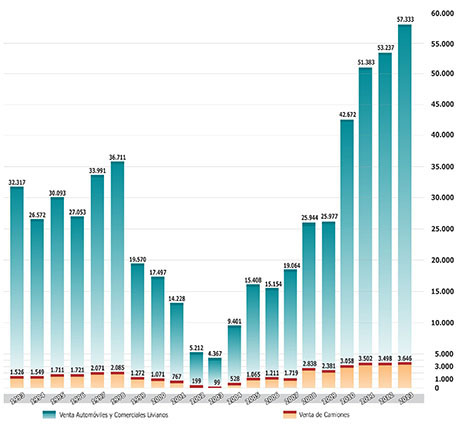
\includegraphics[width=0.9\linewidth]{Figures/ventas_autos}
	\caption[Evolución de la venta de automóviles en Uruguay]{Evolución de la venta de automóviles por año. El valor más bajo corresponde al año 2003, y el más alto 2013. Imagen extraída de {http://www.autoanuario.com.uy}.}
	\label{fig:ventas_autos}
\end{figure}

En un contexto global, el crecimiento en la circulación de automóviles provoca que disminuya el nivel de aceptación del transporte público, cuyo servicio en general es ineficiente. Para resolver este problema las autoridades suelen optar por instrumentar sistemas de transporte costosos como los \emph{metros}, pero se ha demostrado que existen otras opciones viables como el BRT (Bus Rapid Transit / ómnibus de tránsito rápido)\citep{BRT_Dial}.

En el caso de la ciudad de Montevideo, para solucionar este problema se está implementando el Plan de Movilidad Urbana \citep{PlanMovilidad}, con el objetivo de mejorar la eficiencia del transporte público y democratizar el acceso al mismo. El sistema de transporte está inspirado en un BRT, con la construcción de varios corredores exclusivos en la ciudad. En la siguiente sección se presenta más información sobre los BRT, corredores urbanos y en particular el Corredor Garzón.

\section{Corredores urbanos de tráfico}
El corredor urbano de tráfico, también llamado \emph{corredor segregado}, se caracteriza por una separación física entre el carril de circulación de los ómnibus y los carriles para el resto del tráfico. 
Ésta es la principal diferencia con un concepto similar llamado \emph{carril de sólo bus}, en donde se separan los carriles por líneas horizontales pintadas en la calle indicando que sólo pueden circular ómnibus. Los carriles de \emph{sólo bus} suelen ser poco exitosos como medida para agilizar el tráfico de transporte colectivo por falta de control que evite que el tráfico los invada. 

En el caso de Montevideo el carril \emph{sólo bus} está sobre la derecha, por lo que los vehículos privados lo invaden al virar a la derecha y los taxis lo suelen invadir para levantar o dejar pasajeros. Al ubicar los corredores alineados en el medio de las vías de tráfico, se evitan esos problemas.  

Las ciudades de países en vías de desarrollo, que tengan como objetivo fundamental conseguir mayores velocidades en el sistema vial, deben estudiar la factibilidad de instalar corredores, dado que existen muchas posibilidades de implementación y no todas pueden ser aplicables por el contexto zonal, cultural o de inversión necesaria.


BRT es una solución innovadora, de alta capacidad y de menor costo para el transporte público que puede alcanzar el rendimiento y los beneficios de sistemas ferroviarios, con un costo significativamente menor como se puede apreciar en la Figura \ref{fig:Grafica de costos de otros medios de transporte}. Se trata de un sistema integrado de movilidad basado en ómnibus para el transporte de los pasajeros a sus destinos de manera rápida y eficiente. Al mismo tiempo, ofrece la flexibilidad necesaria para satisfacer una variedad de condiciones locales. Los elementos del sistema de BRT pueden ser fácilmente personalizados a las necesidades de la comunidad e incorporan tecnologías de última generación de bajo costo que atraen a más pasajeros y en última instancia ayudan a reducir la congestión de tráfico en general \citep{ITDP}.

\begin{figure}[ht]
	\centering
	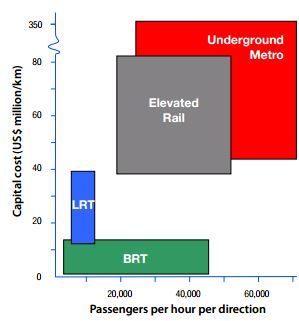
\includegraphics[width=0.9\linewidth]{Figures/costo_transporte}
	\caption[Gráfica de costos de transporte en función de la gente transportada.]{Gráfica de costos de transporte en función de la gente transportada.- Imagen original extraída de \citet{ITDP}		
	}
	\label{fig:Grafica de costos de otros medios de transporte}
\end{figure}

Un BRT contiene características similares al tren ligero o al sistema de metro, por lo que es mucho más confiable, conveniente y rápido que los servicios regulares de ómnibus. Entre sus características fundamentales se destacan el uso de carriles exclusivos para el ómnibus, un alineamiento central del carril y un largo mínimo de 3 km. Además de estás características, se recomienda incluir el uso de ómnibus de gran capacidad para transportar un número mayor de personas, la compra de pasajes fuera del ómnibus (agilizando la entrada de pasajeros) y que el ómnibus tenga prioridad sobre otros vehículos en las intersecciones viales. Con las especificaciones adecuadas, un BRT es capaz de evitar las causas de los retrasos que suelen tener los servicios regulares de ómnibus (como estar atrapado en el tráfico y hacer cola para pagar a bordo). 

Para crear una definición común de BRT y calificar los sistemas existentes alrededor del mundo,  evaluando su funcionamiento basado en las mejores prácticas internacionales, existe el standard BRT creado por \citet{brt_standar}. Su principal objetivo es brindar una mejor experiencia a los pasajeros, con un costo económico acorde e impacto ambiental positivo. Este standard cuenta con un método para calcular el puntaje del corredor y determinar su nivel de calidad. 

En la siguiente sección se presenta un análisis exhaustivo de varios puntos presentados en el standard BRT en relación con el caso de estudio del proyecto: el Corredor Garzón.

	
\section{Corredor Garzón}	


El Corredor Garzón fue construido como parte del Plan de Movilidad Urbana en la ciudad de Montevideo \citep{PlanMovilidad}. El corredor está ubicado en el centro geográfico de Montevideo como se puede apreciar en la Figura \ref{fig:Mapa_Garzon_0} y conecta los barrios de Colón, Sayago, Belvedere y Paso Molino. Tiene una extensión de 6.5 km con 24 cruces semaforizados, en donde se encuentran calles importantes como Millán, que conecta con una autopista (Ruta 5), y Bulevar Batlle y Ordoñez, que tiene una gran densidad de tráfico. Es importante aclarar que el corredor Garzón no es sólo una conexión de extremo a extremo, ya que se encuentra en una zona densamente poblada cuyos barrios tienen al corredor como la principal vía de movilidad.

\begin{figure}
	\centering
	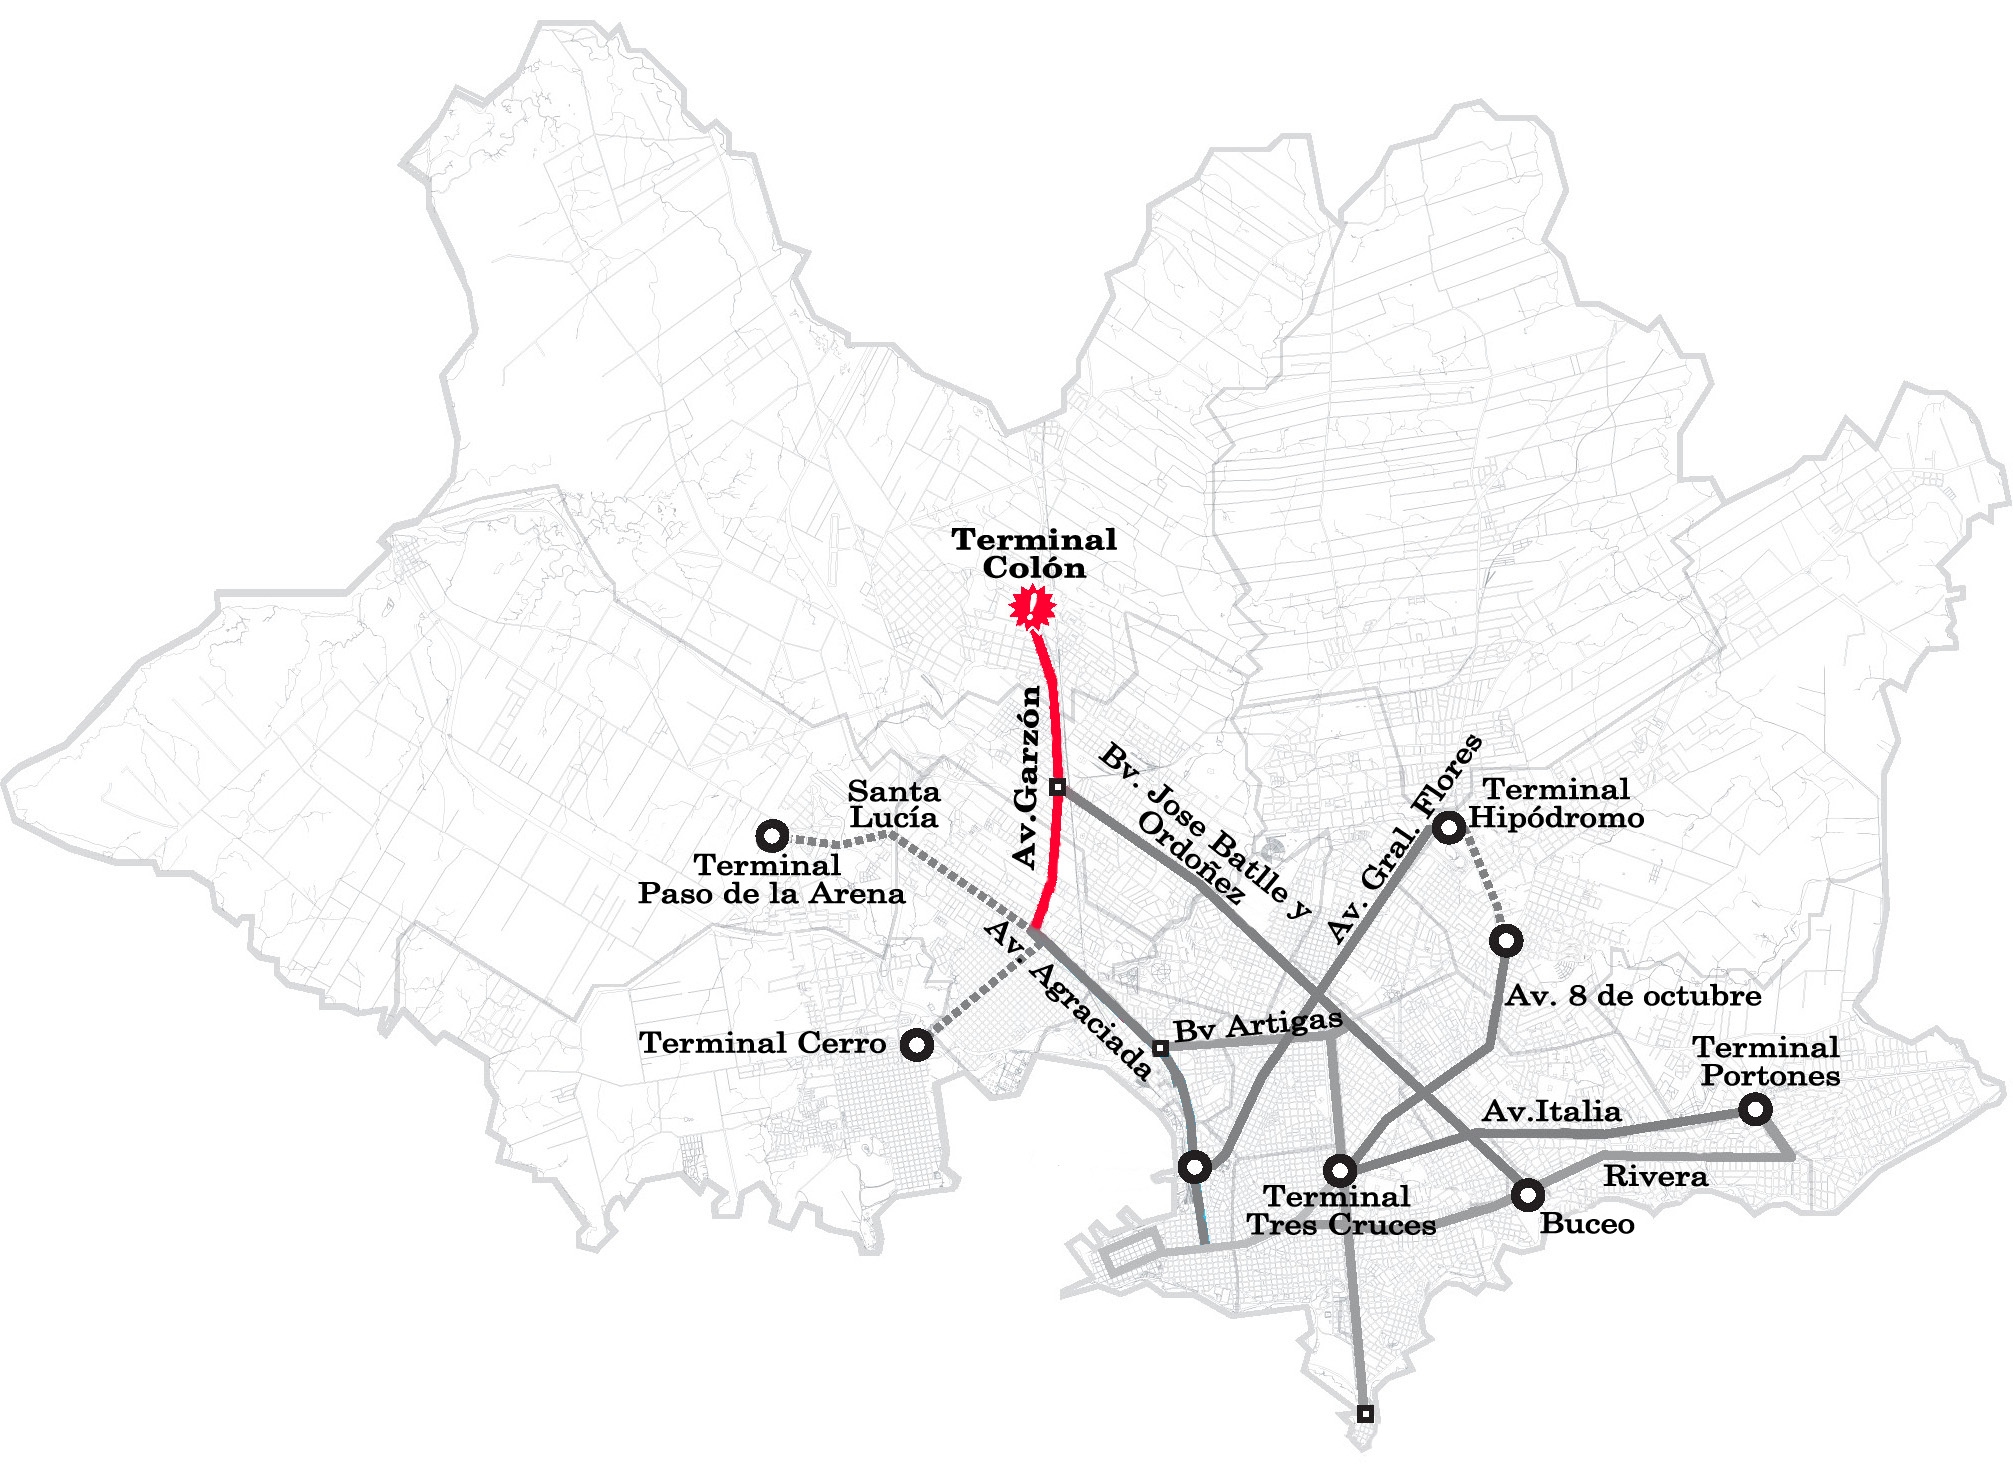
\includegraphics[width=0.99\linewidth]{figures/Mapa_Garzon_0}
	\caption[Localización del Corredor de Garzón en Montevideo]{Localización del Corredor de Garzón en Montevideo, referenciado en color rojo - Imagen original extraída de www.montevideo.gub.uy		
	}
	\label{fig:Mapa_Garzon_0}
\end{figure}

Como se aprecia en la Figura \ref{fig:perfil_garzon}, el corredor consiste básicamente en tres calles paralelas e independientes. Dos calles cuentan con dos carriles de una sola mano y entre medio de éstas se encuentra una calle de doble vía con un carril para cada vía, que es exclusivamente usado por ómnibus urbanos durante el día y por ómnibus urbanos y suburbanos en la noche.

Basándose en el standard antes mencionado, el Corredor Garzón cumple con la definición de BRT por las siguientes características:\textit{i)} el largo del carril exclusivo para los ómnibus es de más de 3 km de longitud,\textit{ii)} más del 90\% de la extensión del corredor está segregado físicamente, impidiendo el traspaso de carril de otros vehículos hacia el carril exclusivo para ómnibus,\textit{iii)} presenta dos carriles centrales para los ómnibus que se encuentran en medio de los carriles para los demás vehículos constituyendo un corredor alineado centralmente,\textit{iv)} incluye prohibiciones de algunos virajes a la izquierda y el carril de ómnibus tiene prioridad en la mayoría de las intersecciones.


\begin{figure}
	\centering
	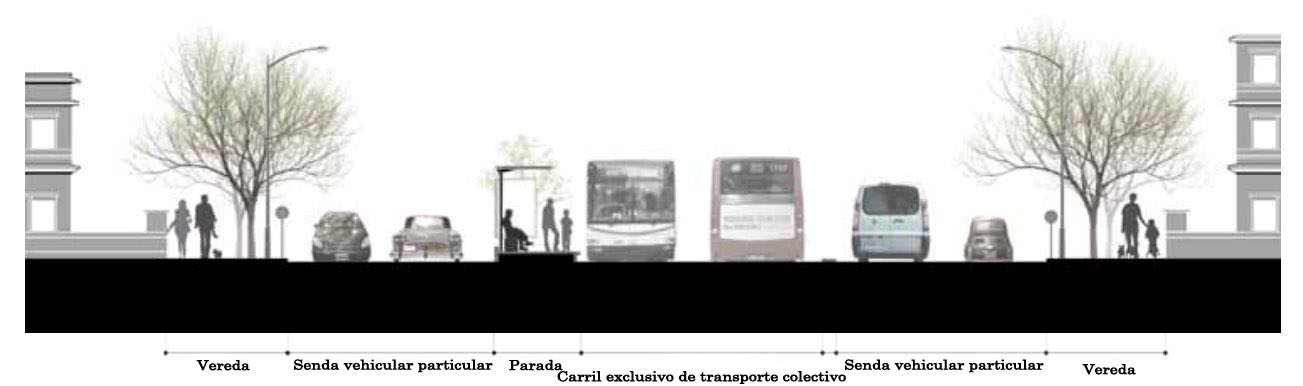
\includegraphics[width=0.9\linewidth]{Figures/busway_configuration}
	\caption[Perfil propuesto para el corredor Garzón.]{Perfil propuesto para el corredor Garzón desde San Quintín a Camino Colman - Imagen original extraída de \citep{PlanMovilidad}
	}
	\label{fig:perfil_garzon}
\end{figure}

\newpage
Analizando los puntos presentados en el standard como recomendaciones para la implementación de corredores urbanos, hay algunas características que no están totalmente aplicadas al Corredor Garzón, entre las que se destacan:

\begin{enumerate}
	\item Cobrar el boleto fuera del ómnibus: uno de los factores más importantes para mejorar la experiencia del usuario, así como también la velocidad en zonas de mucha carga, es que existan al menos algunas estaciones (no sólo paradas de ómnibus) donde el boleto se cobre (o se use tarjeta de transporte) al entrar a la estación.
	\item Ofrecer servicios expresos o limitados: una forma de mejorar las velocidades de operación consiste en crear líneas que no se detengan en todas las paradas (evitando aquellas paradas con menor demanda de pasajeros) y poner más ómnibus en la calle.
	\item Instrumentar un carril extra para adelantarse en paradas: este carril resulta crítico en sistemas de transporte colectivo de gran porte para poder manejar los servicios expresos. En sistemas de baja demanda es una buena inversión y en el caso del Corredor Garzón podría permitir que los servicios suburbanos funcionaran durante todo el día por el corredor, mejorando así el transporte público y privado.
	\item Establecer un mínimo de distancia entre paradas e intersecciones: según el standard, la mínima distancia entre la intersección y la parada es de 26 m, pero idealmente deberían ser 40 m para evitar retrasos. En el Corredor Garzón las paradas están sobre las intersecciones y hay varias paradas donde se detiene más de una línea de ómnibus. Esto puede ocasionar problemas, dado que si uno o dos ómnibus sólo esperan por el semáforo en rojo, los demás que lleguen generarán una fila aguardando para detenerse en la parada y así poder levantar o dejar pasajeros y posiblemente al llegar al cruce ya no los habilitará la luz verde que dejo pasar a los primeros coches, debiendo tener que esperar nuevamente.
	\item Tener estaciones centrales o conexión entre paradas: la ausencia de paradas en el centro de los dos carriles de ómnibus hace que el diseño tenga una construcción más cara (hay que hacer dos paradas). La no existencia de una conexión física para que el pasajero pueda cambiar de recorrido sin tener que cruzar la calle, lo hace menos eficiente y más inseguro.
	\item Contar con una distancia entre estaciones que cumpla el standard:  las paradas deberían estar a una distancia de entre 300 m y 800 m, siendo 450 m la distancia óptima tanto para el pasajero como para el transporte. Si bien el Corredor Garzón cumple la distancia óptima en promedio(464 m), individualmente existen casos como las cuatro paradas que se encuentran entre Emancipación y Avenida Islas Canarias cuyas distancias son menores al mínimo sugerido por el standard.
	\item Utilizar varias puertas para el ingreso/egreso de pasajeros en los ómnibus: con el fin de mejorar el flujo y volumen de pasajeros, sería conveniente contar con dos puertas anchas o al menos tres puertas comunes.
	\item Mejorar la calidad de las paradas: las paradas deberían proteger al usuario de las inclemencias climáticas, contar con puertas corredizas que se abran cuando hay un ómnibus (para evitar que alguien caiga al corredor) y brindar información al pasajero en tiempo real, etc. Estas especificaciones no hacen al corredor más rápido pero si más seguro, cómodo y confiable.
%\item  Semáforos: un corredor debe de funcionar al igual que una autopista, en el sentido de que una vez que se entra debería ser posible mantener la velocidad máxima sin tener que detenerse con frecuencia, por lo que no deberían de haber semáforos cerca uno de otro. De haberlos, la sincronización será la clave para minimizar los tiempos de espera.
%\item Calles paralelas: tener calles paralelas es de vital importancia para un corredor, ya que una de las formas de minimizar los tiempos de espera es prohibir los giros a la izquierda, y una calle paralela provee la facilidad de poder realizarlo.
%\item Giro a la derecha con luz roja: actualmente, en muchos países se encuentra reglamentada una ley que permite a los conductores doblar a la derecha con luz roja, ya que la misma (a menos que se especifique) es tomada como un cartel de pare \emph{solamente} para doblar a la derecha. En donde esta aprobada esta ley acorta los tiempos de luz verde de las transversales, mejorando así la velocidad promedio en los corredores o calles importantes.
\end{enumerate}

Desde su inauguración en el año 2012, el corredor ha recibido críticas debido a que su principal objetivo de agilizar el transporte público no fue cumplido. Luego de varios intentos de mejoras al respecto, se ha vuelto a una situación que implica la misma velocidad promedio para el transporte público que existía antes de realizar el corredor \citep{olivera2015}.

Las autoridades municipales admitieron que se han cometido errores en el diseño del corredor, y que no se ha logrado sincronizar los semáforos en las vías de tránsito que lo componen \citep{olivera2013}. Un buen funcionamiento de los semáforos es fundamental para asegurar que el tráfico circule con eficiencia y a la vez aporte seguridad a los peatones. A continuación se tratará específicamente el tema de la sincronización de semáforos, que da la motivación para este proyecto. 


\section{Sincronización de semáforos}
Los métodos utilizados para la optimización del tráfico tienen como objetivo mejorar el flujo de vehículos en una red vial. Estos métodos se pueden clasificar en dos categorías: los que influyen en el comportamiento de los conductores (mediante la configuración de semáforos, introducción de señalizaciones, etc) o los que realizan modificaciones en las vías de tráfico (agregando nuevos carriles, ensanchando calles, etc). Las modificaciones de infraestructuras pueden producir mejoras drásticas, pero requieren una inversión monetaria y un espacio físico que muchas veces no está disponible. Por esta razón, los métodos destinados a influir en el comportamiento de los conductores se presentan como una mejor opción o inclusive como única opción en muchos escenarios.

Los métodos para la sincronización de semáforos se encuentran entre los más efectivos para agilizar el tránsito y no generar congestiones. Estas técnicas permiten aumentar la velocidad promedio de los viajes y mejorar las perspectivas de desarrollo de la ciudad así como la calidad de vida de sus habitantes. 

Un concepto importante en el manejo de semáforos es el de \emph{fase}, que se refiere a una configuración específica de luces de semáforos en una intersección de calles, que permiten el movimiento de ciertos flujos de tráfico. Como se ve en la Figura \ref{fig:fases} cada intersección puede tener diferente número de fases y también distintas duraciones. Las fases suelen ser configuradas y establecidas manualmente por técnicos especializados basados en su experiencia, aunque en ciertas ocasiones se utilizan simulaciones computacionales para obtener configuraciones apropiadas. 

\begin{figure}
	\centering
	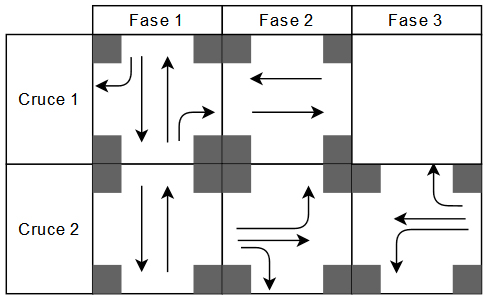
\includegraphics[width=0.8\linewidth]{Figures/fases1}
	\caption{Distintas fases de semáforos para dos cruces en una red de tránsito.}
	\label{fig:fases}
\end{figure}

Existen tres parámetros a tener en cuenta, que determinarán el comportamiento del sistema: la duración de fase, los ciclos de las luces y los valores de \emph{offset}. 
A continuación se explica cada uno de ellos:


\begin{itemize}
 	\item Duración de fase: Se refiere a la duración en que una configuración específica de las luces de los semáforos está activa en una intersección. Un conjunto de las luces estará en verde y otras en rojo, determinando qué vía se encuentra habilitada para cruzar en ese momento. La elección correcta de este parámetro es fundamental para lograr fluidez en el tránsito; las calles con una densidad de tránsito mayor tendrían que tener más tiempo asignado para cruzar. Realizar la optimización individual de cada intersección no tiene por qué conducir a una solución óptima de toda la red vial, ya que puede ocasionar cambios en el flujo vehicular que afecte otras secciones de la red. Por esta razón es conveniente utilizar un enfoque global al modelar una solución.
 	
 	\item Duración del ciclo: Un ciclo representa un conjunto de fases. En general la duración de un ciclo es la suma de las duraciones de las fases. Como indica su nombre, el ciclo se repetirá una vez que se completa. La duración puede incrementarse o decrementarse para permitir mayor cantidad de repeticiones de las fases.
 	% Otro punto a considerar, sobre todo en intersecciones complejas, es el orden en el cual las fases son ejecutadas.
 	
 	\item \emph{Offset}: Indica en qué fase comienza el ciclo o en qué instante de tiempo, permitiendo que las intersecciones comiencen su ciclo en diferentes momentos. Este concepto es muy importante para sincronizar un flujo de tráfico en lo que se conoce como \emph{línea verde}, en donde los vehículos logran pasar todas las intersecciones sin detenerse.
\end{itemize}

Los parámetros mencionados anteriormente pueden ser utilizados a la hora de sincronizar los semáforos de una zona, buscando una optimización global de la red vial. También se debe tener en cuenta la implementación de soluciones seguras desde el punto de vista de las ordenanzas de tránsito, siendo lo más básico que no existan intersecciones donde los flujos vehiculares estén habilitados para cruzar al mismo tiempo.

Los métodos para lograr la coordinación necesaria entre semáforos incluyen desde simples mecanismos de reloj hasta sistemas computarizados que se ajustan en tiempo real con la ayuda de sensores en la calle. Estos métodos pueden clasificarse como estrategias de tiempo fijo o de tiempo dinámico auto-ajustable.

Se considera al problema de sincronización de semáforos como un problema de optimización NP-difícil \citep{yang1996model}, lo que provoca que los métodos computacionales exactos lo resuelvan eficientemente solamente en instancias de tamaño reducido. Por este motivo deben utilizarse métodos heurísticos y metaheurísticos para resolver instancias realistas del problema, algunos de los cuales se describen en la sección de trabajos relacionados. Entre los métodos más desarrollados y efectivos para resolver el problema están los algoritmos evolutivos, en particular los algoritmos genéticos, que serán explicados a continuación.

\section{Algoritmos Evolutivos}

Los Algoritmos Evolutivos (AE) son un conjunto de técnicas metaheurísticas para la resolución de problemas complejos que se inspiran en la evolución natural. Los AE trabajan sobre una población de individuos que representan una solución y utilizan mecanismos de selección, reproducción y técnicas para mantener la diversidad para calcular soluciones de buena calidad para el problema \citep{spears2000evolutionary}. 

Un AE se describe como una técnica iterativa que busca en cada paso mejorar las soluciones por medio de operadores de exploración y explotación, basado en un criterio predefinido a maximizar o minimizar.

Se pueden destacar cuatro etapas en la ejecución del AE:

\begin{itemize}
	\item Evaluación: Para cada individuo de la población se determina un valor de aptitud \emph{fitness} en relación a su capacidad para resolver el problema. 
	\item Selección: Proceso en donde se eligen cuales son los individuos que sobrevivirán a la siguiente generación y sobre los cuales se aplicarán los operadores evolutivos.
	\item Operadores evolutivos: Se aplican combinaciones entre individuos (cruzamiento), y modificaciones aleatorias de individuos(mutación). Los operadores generan nuevos individuos que sustituirán a los existentes en la población.
	\item Reemplazo: Se produce el recambio generacional, sustituyendo a la antigua población por una nueva que podría tener sobrevivientes de la anterior o solamente nuevos individuados generados en la etapa de aplicación de los operadores evolutivos.
\end{itemize}

Se han desarrollado enfoques de algoritmos de optimización que aplican estos conceptos, las más relevantes se describen a continuación:

\begin{itemize}

	\item Estrategias de Evolución: Propuesto por \citet{Ingo1971}, fue originalmente propuesto como un método de optimización utilizando individuos que codifican números reales en problemas relacionados al diseño de ingeniería. Su característica principal es que utilizan el operador de mutación como motor para la evolución. Sin embargo, modelos más recientes agregan otro tipo de operadores, incluyendo cruzamiento.
	\item Programación genética: Intenta generar un programa de computación para resolver una tarea específica, aplicando técnicas evolutivas. Cada individuo puede ser un programa que es representado en forma de árbol, donde cada nodo del árbol tiene una operación y los nodos terminales un operando, de esta manera se facilita la evaluación de expresiones matemáticas. La función de aptitud se refiere a qué tan cerca de resolver la tarea se encuentra el individuo \citep{Koza1992}.
	\item Algoritmo Genético: Es considerado el más popular de los AE, dado su versatilidad a la hora de resolver problemas de optimización. El operador de cruzamiento es el principal operador evolutivo siendo el de mutación un operador secundario. Estos operadores se aplican sobre la población de soluciones potenciales en cada generación. En la siguiente sección se presentan en detalle las características de los algoritmos genéticos (AG), que es la técnica que se utiliza en este trabajo para resolver el problema de sincronización de semáforos.
	
\end{itemize}

\subsection{Algoritmos Genéticos}
En Algoritmo \ref{alg:algoritmo_genetico_simple} muestra la formulación básica de un algoritmo genético (AG) que se basa en el esquema general de un AE. Comienza con una población inicial de individuos a los cuales en cada generación se le aplican operadores de cruzamiento y mutación, seleccionando a los mejores en base a su aptitud para resolver el problema. El operador de cruzamiento guía la búsqueda, mientras el operador de mutación se encarga de aportar diversidad a la exploración. Por tanto el objetivo es que con el paso de las generaciones se obtengan mejores soluciones, como se muestra la Figura \ref{fig:fitness_generaciones} hasta detenerse usando un criterio de parada, ya sea el número de iteraciones o cuando ya no se puede mejorar más la solución. Los trabajos de \citet{Goldberg1989} y \citet{Mitchell1996} brindan más detalles sobre los AE.

\subsubsection{Esquema del algoritmo}

El esquema básico de funcionamiento se presenta en el Algoritmo \ref{alg:algoritmo_genetico_simple}:


\begin{algorithm}[ht]
	\caption{Algoritmo Genético}
	\label{alg:algoritmo_genetico_simple}
	\begin{algorithmic} [1] 
		{
			%\small
			\STATE {Inicializar(Pob(0))}
			\STATE {generación} = 0
			\STATE \textbf{mientras} {no se cumple el criterio de parada} \textbf{hacer}
			\STATE\hspace{\algorithmicindent} {Evaluar (Pob(generación))}
			\STATE\hspace{\algorithmicindent} {Padres = Seleccionar(Pob(generación))}
			\STATE\hspace{\algorithmicindent} {Hijos = Cruzamiento(Padres)}
			\STATE\hspace{\algorithmicindent} {Hijos = Mutación(Hijos)}
			\STATE\hspace{\algorithmicindent} {NuevaPob = (Reemplazar Pob(generación), Hijos)}
			\STATE\hspace{\algorithmicindent} {generación}++
			\STATE \textbf{fin}
			\STATE \textbf{retornar} mejor solución encontrada
		}
	\end{algorithmic}
\end{algorithm}


Un individuo es una codificación de una solución que resuelve el problema. La población inicial puede generarse aleatoriamente o basándose en heurísticas que utilizan conocimiento específico sobre el problema. El mecanismo de selección determina cuales individuos son adecuados para integrar la población de la siguiente generación. Este mecanismo utiliza el valor de la función de evaluación o \emph{fitness} para definir que tan buena o apta es una solución en comparación con las demás. En cada iteración, la cual se conoce como generación, se aplican operadores de cruzamiento y mutación sobre los individuos. El cruzamiento permite combinar a dos individuos para obtener otros que potencialmente sean una mejor solución. La mutación aplica cambios aleatorios sobre los individuos. Estos operadores y el mecanismo de selección son probabilísticos, es decir, que su aplicación depende de una una tasa de probabilidad asociada al operador.


\begin{figure}[ht]
	\centering
	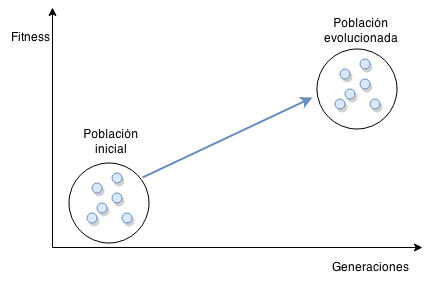
\includegraphics[width=10cm]{Figures/fitness_generaciones}
	\caption[Esquema de la evolución del valor del fitness en un algoritmo evolutivo ]{Esquema de la evolución del valor del fitness en un algoritmo evolutivo a través de las generaciones.}
	\label{fig:fitness_generaciones}
\end{figure}

Por tanto se van seleccionando, combinando y cambiando las mejores soluciones en un proceso, que si el AG está bien diseñado, permite ir obteniendo mejores soluciones.
El criterio de parada nos indica cuando termina este proceso, ya sea porque se alcanzó un número de generaciones predefinidos o porque la mejora no es evidente. Al final se devuelve la mejor solución encontrada en todo el proceso.

%Hay que indicar que no es una técnica exacta pero logra muy buenas aproximaciones, además se aplica en problemas complejos por su flexibilidad y robustez. 

A continuación se presentan las principales características de los AG.




\subsubsection{Representación de soluciones}
%Dado que no se puede trabajar directamente sobre las soluciones, estas se codificaron en un modelo donde es posible aplicar el algoritmo.
Los AG no trabajan directamente sobre las soluciones del problema, sino que utilizan una abstracción de las soluciones llamada cromosoma. Un cromosoma es un vector de genes donde el valor de cada gen se denomina alelo; nombres inspirados en la evolución natural biológica.
En general los AG codifican las soluciones utilizando un vector de números binarios o reales de largo fijo.

\begin{figure}[ht]
	\centering
	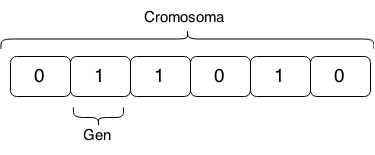
\includegraphics[width=8cm]{Figures/rep_binaria}
	\caption{Representación binaria de un cromosoma.}
	\label{fig:rep_binaria}
\end{figure}


\subsubsection{Función de Evaluación} 
La función de evaluación indica qué tan bueno es un individuo para resolver el problema en cuestión, utilizando un valor conocido como \emph{fitness}, por lo que también es llamada función de \emph{fitness}. Este valor se utiliza para definir cuales son los mejores individuos y de esta forma guiar la exploración hacia la región que incluya las mejores soluciones. En general, la función de \emph{fitness} es la que insume la mayor cantidad de tiempo del algoritmo genético, en comparación con los demás operadores.

\subsubsection{Operador de Selección}
Existen diversos operadores de selección, cuya función es mantener las mejores características de los individuos en las siguientes generaciones. Entre ellos se encuentran:
\begin{itemize}
	\item Selección proporcional: Elige aleatoriamente individuos donde la probabilidad de selección es proporcional al valor del \emph{fitness}. Los mejores individuos son elegidos con mayor probabilidad, pero los peores individuos también pueden ser elegidos, lo que permite mantener la diversidad en la población. Sea N la cantidad de individuos en la población y $f_i$ el valor de \emph{fitness} del i-ésimo individuo, la probabilidad asociada a su selección está dada por la la ecuación \ref{eq:seleccion_proporcional} .
	\item Torneo: Se eligen aleatoriamente un determinado número de individuos y se selecciona un subconjunto de los individuos con mejor \emph{fitness}.
	\item Rango: Se ordenan los individuos por el valor de \emph{fitness} y se selecciona un determinado porcentaje(rango) de los mejores individuos.
\end{itemize}

\begin{equation}
\label{eq:seleccion_proporcional}
F(x) =  p_i = \frac{f_i}{\sum_{j=1}^{n}{f_j}}  
\end{equation}
        
        
\subsubsection{Operador de cruzamiento}
La función del operador de cruzamiento es combinar individuos con el objetivo de preservar las mejores características de los progenitores y así lograr construir mejores soluciones. El operador de cruzamiento se aplica de acuerdo a una tasa de probabilidad prefijada. 


En general, los operadores de cruzamiento se pueden clasificar en:

\begin{itemize}
	\item Cruzamiento de un punto: A partir de dos padres se selecciona un punto al azar de los cromosomas obteniendo dos trozos que se combinan para obtener dos hijos. Se explica en la Figura ~\ref{fig:cruzamiento1}
	\item Cruzamiento multipunto: El método anterior se puede generalizar para obtener más puntos de corte y más recombinaciones.
	\item Cruzamiento uniforme: Para cada posición en el cromosoma se   intercambian genes según una tasa de probabilidad, este mecanismo se muestra en la Figura \ref{fig:cruzamiento_uniforme} .	
\end{itemize}

\begin{figure}[ht]
	\centering
	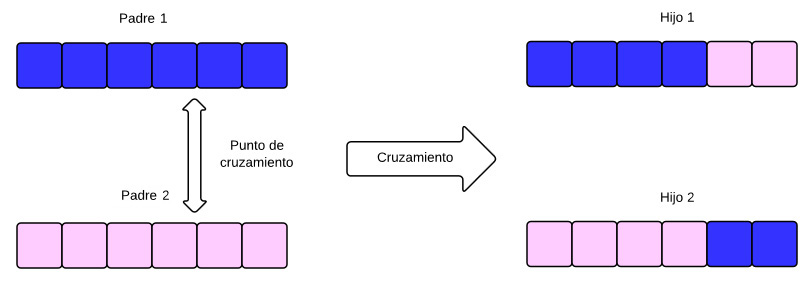
\includegraphics[width=\textwidth]{Figures/cruzamiento1}
	\caption{Cruzamiento de un punto}
	\label{fig:cruzamiento1}
\end{figure}

\begin{figure}[ht]
	\centering
	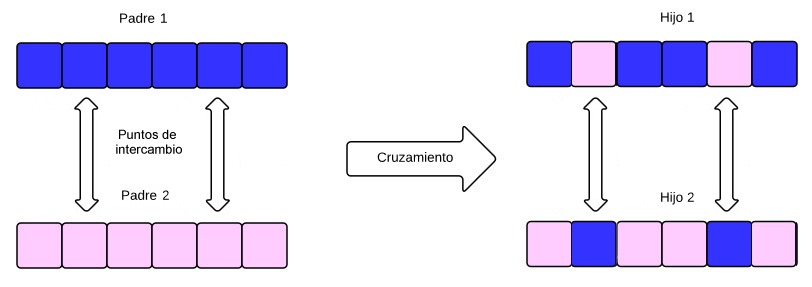
\includegraphics[width=\textwidth]{Figures/cruzamiento_uniforme}
	\caption{Cruzamiento uniforme}
	\label{fig:cruzamiento_uniforme}
\end{figure}

\subsubsection{Operador de mutación} 
El operador de mutación es el método utilizado para modificar un individuo, con el objetivo de mantener y mejorar la diversidad y otorgar al AG un mecanismo que le permita escapar de óptimos locales. En general la mutación aplica una modificación aleatoria en el cromosoma, por ejemplo, en una representación binaria se invertiría aleatoriamente el valor de un alelo, como se muestra en la Figura \ref{fig:mutacion1}.
\begin{figure}[ht]
	\centering
	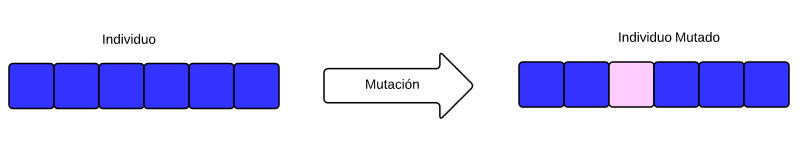
\includegraphics[width=1\linewidth]{Figures/mutacion1}
	\caption{Mutación por inversión binaria}
	\label{fig:mutacion1}
\end{figure}


\subsubsection{Criterio de reemplazo} 
El criterio de reemplazo indica cual es el mecanismo utilizado para realizar el recambio generacional. Se podría reemplazar todos los padres por los hijos o seleccionar sólo algunos padres a reemplazar, que en general son los que tienen peor valor de \emph{fitness}).

\subsubsection{Criterio de parada} 
El criterio de parada indica cuándo debe terminar la fase iterativa del algoritmo. Puede definirse un número prefijado de generaciones o determinar si el proceso se estanca, por ejemplo cuando no se generan mejoras significativas en el valor de \emph{fitness}.



% ctrl+t comenta
%\begin{algorithm}%[!ht]
%	\caption{Genetic Algorithm}
%
%	\begin{algorithmic} [1] 
%		{
%
%			\STATE {Init( Pop(0))}
%			\STATE \texttt{generation} = 0
%			\WHILE {\text{NOT Stop Criteria}}
%			\STATE {Evaluate Pop(generation)}
%			\STATE {Parents = Selection(Pop(generation))}
%			\STATE {Children = Crossover(Parents) and Mutation(Parents)}
%			\STATE {NewPop = Replace Pop(generation) with Children}
%			\STATE \texttt{generation}++
%			\ENDWHILE
%			\RETURN Best solution
%		}
%	\end{algorithmic}
%\end{algorithm}


\subsection{Algoritmos evolutivos multiobjetivo}

Los problemas de optimización multiobjetivo trabajan sobre un espacio multidimensional de funciones y no tienen una única solución. Por este motivo, el significado de óptimo cambia. Una solución es un \emph{óptimo de Pareto} si ninguna de las funciones objetivo puede mejorar su valor sin degradar otro de los valores objetivo. Todas estas soluciones son consideradas igualmente buenas, ya que los vectores no se pueden ordenar completamente y representan diferentes valores de compromiso entre las funciones objetivo. Al conjunto de los valores funcionales de los óptimos de Pareto se les llama frente de Pareto.

Existen algoritmos evolutivos para resolver problemas de optimización multiobjetivo. Éstos son los llamados MOEA, por sus siglas en inglés \emph{ MultiObjetive Evolutionary Algorithm}. Sus propósitos son aproximarse al frente de Pareto y lograr obtener una gama de diferentes compromisos entre las funciones a optimizar para luego poder tomar la decisión de cual elegir. Para un análisis más detallado de los AE multiobjetivo se recomienda el trabajo de \citet{Deb2001}.


El Algoritmo \ref{alg:algoritmo_genetico_multiobjetivo} describe el esquema básico de un MOEA, donde se aprecia que existen dos operadores característicos: el operador de diversidad y el operador de asignación de \emph{fitness}. El primero se aplica para evitar la convergencia a un sector en particular del frente de Pareto, mientras que el segundo intenta brindar mayor chance de perpetuar a los individuos con mejores características.

\begin{algorithm}[ht]
	\caption[Algoritmo evolutivo multiobjetivo]{Algoritmo evolutivo multiobjetivo. En negrita se indican las diferencias con el algoritmo evolutivo genérico.}
	\label{alg:algoritmo_genetico_multiobjetivo}
	\begin{algorithmic} [1] 
		{
			%\small
			\STATE {Inicializar(Pob(0))}
			\STATE {generación} = 0
			\STATE \textbf{mientras} {no se cumple el criterio de parada} \textbf{hacer}
			\STATE\hspace{\algorithmicindent} {Evaluar (Pob(generación))}
			\STATE\hspace{\algorithmicindent} \textbf{Operador diversidad(Pob(generación))}
			\STATE\hspace{\algorithmicindent} \textbf{Asignar fitness(Pob(generación))}						
			\STATE\hspace{\algorithmicindent} {Padres = Seleccionar(Pob(generación))}
			\STATE\hspace{\algorithmicindent} {Hijos = Cruzamiento(Padres)}
			\STATE\hspace{\algorithmicindent} {Hijos = Mutación(Hijos)}
			\STATE\hspace{\algorithmicindent} {NuevaPob = (Reemplazar Pob(generación), Hijos)}
			\STATE\hspace{\algorithmicindent} {generación}++
			\STATE \textbf{fin}
			\STATE \textbf{retornar} \textbf{frente de pareto}
		}
	\end{algorithmic}
\end{algorithm}

Los MOEA se pueden clasificar por el método de asignación de \emph{fitness}. Por un lado se tienen los que no son basados en Pareto, que utilizan métodos sencillos de asignación de \emph{fitness}. Estos métodos no reflejan la independencia entre los objetivos y tampoco garantizan una resolución correcta del problema. Un método popular entre los que no utilizan dominancia de Pareto es la combinación lineal de los objetivos, que es relativamente sencilla de implementar y adecuada para problemas de optimización con no más de tres funciones objetivo y donde el frente de Pareto del problema es convexo \citep{coello2002evolutionary}. En este caso el problema es tratado como una optimización monoobjetivo, no reflejando el carácter multiobjetivo.  En este método, el \emph{fitness} se calcula como una suma ponderada, con los pesos fijados a priori, de acuerdo a la expresión en la Ecuación \ref{eq:funcion_fitness_generica}.

\begin{equation}
\label{eq:funcion_fitness_generica}
F(x) = \sum_{i=1}^{n}{w_i}{f_i}(x)
\end{equation}

%El enfoque de agregación ha sido utilizado en otros trabajos de sincronización de semáforos (cuáles?) y también ha sido utilizado en la resolución de problemas de optimización multiobjetivo relacionados con el manejo inteligente de problemas de tránsito en ciudades modernas (smart cities).

Por otro lado, se encuentran los métodos de asignación de fitness que utilizan explícitamente la dominancia de Pareto y garantizan la  independencia entre los objetivos del problema.   

\subsection{Algoritmos evolutivos paralelos}
Resolver problemas complejos suelen insumir gran cantidad de tiempo, por lo que paralelizar el AE es útil para lograr tiempos de ejecución menores. Pero éste no es el único objetivo que se puede conseguir con un AE paralelo, entre otros existen: encontrar soluciones alternativas al mismo problema, búsqueda más eficiente aún sin \emph{hardware} paralelo, facilidad en la cooperación con otros métodos y búsqueda paralela de múltiples puntos en el espacio \citep{Alba2002}. 

En el caso de los AG, gran parte del tiempo se ocupa en la etapa de evaluación de \emph{fitness}, por esta razón es un buen método distribuir la carga en varios procesadores para que las evaluaciones se realicen en paralelo. 

Un modelo de AE paralelo muy utilizado por su facilidad conceptual y facilidad de implementación es el \emph{maestro-esclavo} que brinda la posibilidad de utilizar racionalmente los recursos computacionales disponibles en todos los computadores modernos. El proceso maestro es el encargado de ejecutar los operadores básicos del algoritmo y distribuir a procesos esclavos la evaluación de  fitness para un conjunto de individuos. El esclavo devuelve el resultado y luego el maestro es el encargado de continuar con la evaluación, ejecutando los operadores. De este modo aumenta la eficiencia computacional del algoritmo ya que las múltiples ejecuciones de una de las funciones más costosas es distribuida entre varios procesos que ejecutan concurrentemente.

\begin{figure}[ht]
	\centering
	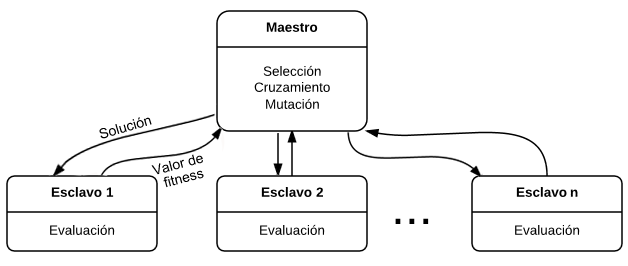
\includegraphics[width=0.9\linewidth]{Figures/diagrama-master-slave}
	\caption[Modelo Maestro-Esclavo]{Modelo Maestro-Esclavo}
	\label{fig:diagrama-master-slave}
\end{figure}

\subsection{Implementación y entornos de desarrollo}

A la hora de implementar un AG es importante tener en cuenta ciertos aspectos que dotarán a la solución de una mayor flexibilidad, eficiencia y robustez. En general se recomienda usar el paradigma de orientación a objetos, ya que aporta múltiples ventajas entre las que se encuentran: reusabilidad del código, abstracción de problemas, modularidad y legibilidad. Sin embargo, la orientación a objetos puede ocasionar pérdidas de eficiencia computacional, por lo que hay que balancear estos aspectos.

En el trabajo de \citet{Alba1997} se indican con más detalle los elementos importantes de una implementación de AG, entre ellos se destacan: no utilizar tamaño fijo para las poblaciones pues afectan la flexibilidad, evitar las múltiples evaluaciones de una misma solución, dar al usuario la posibilidad de extender las funcionalidades de manera modular, al implementar bibliotecas genéricas usar lenguajes orientados a objetos que permiten su extensión en forma sencilla. Por estas razones se han desarrollado entornos de desarrollo o \emph{frameworks} para trabajar en la resolución de problemas utilizando AE y otras técnicas metaheurísticas. Los \emph{frameworks} encapsulan de manera transparente al usuario los aspectos antes mencionados, lo que permite un desarrollo más rápido, sencillo y seguro.

Existe una gran variedad de \emph{frameworks} para AE; a continuación se describen algunos de los más populares junto con sus principales características.

\begin{itemize}
	\item JMetal: Es un \emph{framework} orientado a objetos basado en Java para la resolución de problemas de optimización multiobjetivo utilizando metaheurísticas. Su arquitectura permite experimentar con técnicas embebidas y también desarrolladas por el usuario. Entre sus características se destaca que al estar implementado en Java puede ser usado tanto en sistemas Windows como Linux. Posee una amplia variedad de algoritmos multiobjetivo listos para usar, y también algoritmos paralelos. Está en constante desarrollo y posee una documentación detallada \citep{Jmetal}.
	
	\item Galib: Es una biblioteca escrita en C++ que incluye objetos y herramientas útiles para la resolución de problemas usando AG. Es gratuita y de código abierto, pudiendo ser ejecutada tanto en Linux como en Windows. No tiene un desarrollo sostenido, siendo su última actualización en el año 2000, esto no quita que todavía se siga usando por su sencillez y flexibilidad \citep{Galib}.
	
	\item Paradiseo: Es un \emph{framework} orientado a objetos que utiliza C++. Su objetivo es el diseño de metaheurísticas tanto paralelas como distribuidas. Cuenta con AE, búsquedas locales y optimización basada en enjambres. Funciona tanto en plataformas Windows como Linux y posee varios módulos destinados a extender sus funcionalidades. Tiene una buena documentación y su ultima versión data del año 2012 \citep{Paradiseo}.
	
	\item Open Beagle: Es un \emph{framework} en C++ que utiliza AE. Brinda un entorno de alto nivel para trabajar con distintas técnicas, soporta programación evolutiva, AG y estrategias evolutivas. Su arquitectura permite utilizar los principios de la programación orientada a objetos para lograr un código recusable y eficiente. Sus características apuntan a brindar un entorno amigable, eficiente, multi-plataforma y gratuito \citep{OpenBeagle}.
	
	\item Mallba: Es una biblioteca escrita en C++ que brinda esqueletos de algoritmos exactos, metaheurísticas, e híbridos para la resolución de problemas de optimización. Mallba maneja el paralelismo de forma simple para el usuario. Posee una arquitectura flexible y extensible lo que permite agregar nuevos esqueletos de forma simple. No cuenta con documentación extensa pero si con varios ejemplos completos de implementaciones de los algoritmos. Mallba funciona tanto en ambiente Linux como Windows \citep{Mallba}.
	
	\item Malva: Surge como un \emph{branch} de la biblioteca Mallba, con modificaciones para ser ejecutado en ambientes actuales, por lo que cuenta con las mismas características aunque al estar en fase de desarrollo soporta sólo algunos algoritmos, entre ellos AG \citep{Malva}.
\end{itemize}

Los \emph{frameworks} son una herramienta importante a la hora de desarrollar un AE. Al enfocarse en el problema de la sincronización de semáforos también serán necesarias otras utilidades entre las que se encuentra los simuladores de tráfico, los cuales serán explicados en la siguiente sección.


\section{Simulación de tráfico}

Los simuladores de tráfico son programas que simulan el movimiento del flujo vehicular sobre una red terrestre, marítima o aérea. Son usados en proyectos de investigación, estudio de congestiones y análisis de impacto de obras.  Existen varias razones para optar por esta herramienta, entre las que se encuentran: la rapidez en la obtención de resultados y el costo asociado de implementación.

% la rapidez en la obtención de resultados ya que la simulación se puede realizar en tiempos mucho más rápidos que en la realidad, el costo, pues no es necesario cambiar la infraestructura para probar nuevos escenarios y es útil para prever situaciones que podrían darse bajo determinadas circunstancias.

Los simuladores se pueden dividir en dos grandes categorías, macroscópicos y microscópicos. En algunos casos se considera una tercera categoría híbrida de estas dos llamada mesoscópicos. En los simuladores \emph{macroscópicos} el tráfico es modelado como un flujo continuo y es descrito de manera agregada usando características como la velocidad o densidad del flujo. En los simuladores \emph{microscópicos} el tráfico se considera compuesto de partículas discretas. Cada partícula es actualizada según las propiedades de la red en ese momento, como límites de velocidad, vehículos cercanos y caminos a seguir. Los simuladores microscópicos utilizan un modelo de decisiones del conductor, lo que permite crear una distribución heterogénea del comportamiento de los vehículos. En general, los simuladores \emph{mesoscópicos} representan a los individuos con alto nivel de detalle pero sus interacciones y actividades con un bajo nivel de detalle, por ejemplo, agrupando vehículos en paquetes que se mueven por una red, considerándolos como una sola entidad.


Se considera que las simulaciones microscópicas se aproximan más a la realidad y que obtienen un nivel de granularidad mayor. Estas características pueden ser útiles cuando se asignan propiedades sobre cada vehículo y se quiere observar el comportamiento cuando éstas cambian. Sin embargo, no implica que se dejen de usar simulaciones macroscópicas, pues aunque no poseen tanto detalle son más rápidas y en determinadas circunstancias podrían ser una mejor opción.

En la actualidad existe una gran variedad de simuladores disponibles, que se encuentran en las diferentes categorías que fueron mencionadas anteriormente. A continuación se ofrece una breve descripción de algunos de los simuladores presentados en el trabajo de \citet{review_trafico} que presenta una lista detallada de simuladores de tráfico.
\begin{itemize}
	\item SUMO: Simulador abierto, portable, microscópico diseñado para soportar grandes redes de tránsito. Es de los más populares, y utiliza una serie de archivos de configuración para representar las rutas, los vehículos y el tráfico \citep{SUMO}.
	\item QuadStone Paramics Modeller: Simulador modular y microscópico capaz de modelar un amplio rango de problemas de tránsito y transporte.
	\item Aimsun: Paquete de simulación que integra varios tipos de modelos de transporte, por ejemplo herramientas para el tráfico estático y un simulador microscópico
	\item Trafficware SimTraffic: Es un simulador que forma parte del paquete \emph{Trafficware's Syncro Studio}, que cuenta con una herramienta para la sincronización de semáforos.
	\item Corsim Trafvu: Parte del paquete \emph{Tsis Corsim}, presenta las animaciones y los gráficos estáticos para las redes de tráfico utilizando \emph{Corsim} como entrada.
\end{itemize}

Cabe destacar que de los cinco simuladores de tráfico mencionados anteriormente, solamente SUMO es abierto y gratuito, el resto son programas propietarios. 

\begin{figure}[ht]
	\centering
	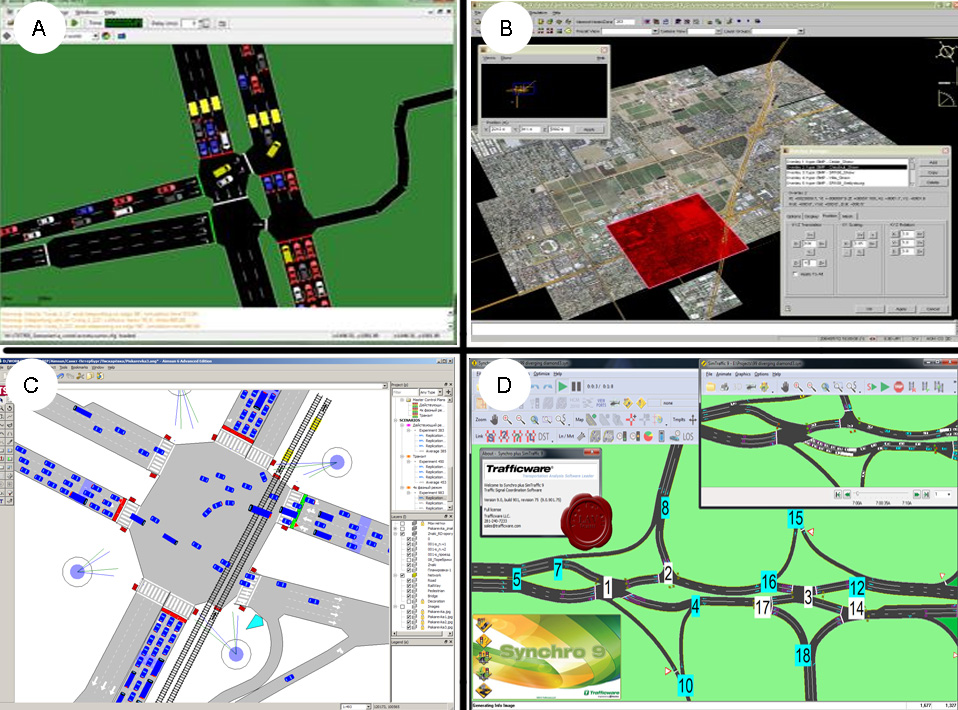
\includegraphics[width=0.9\linewidth]{Figures/simuladores}
	\caption[]{Algunos simuladores de tráfico. (A) Sumo, (B) QuadStone Paramics, (C) Aimsun, (D) Trafficware SimTraffic}
	\label{fig:simuladores}
\end{figure}

Los simuladores requieren de la creación de una \emph{red de tránsito}. En general, la red refiere a las propiedades que tendrán las vías de tránsito, por ejemplo: la cantidad de carriles, el límite de velocidad, la ubicación, el largo, las conexiones entre calles, etc. Algunos simuladores obtienen esta entrada desde archivos de texto, lo cual puede ser un proceso lento y propenso a errores; otros pueden importar redes viales de servicios, como Open Street Map \citep{OSM}. También necesitan conocer las\emph{ rutas seguidas por los vehículos}. Los simuladores pueden tomar esta información de manera explícita, indicando para cada vehículo la ruta seguida, o utilizando otros métodos dinámicos indicando sólo los puntos de inicio y final del recorrido, cuya ruta será generada en tiempo de simulación. El procesamiento manual para generar los recorridos vehiculares puede ser un proceso verdaderamente complejo, por este motivo muchos simuladores brindan herramientas destinadas a facilitar esta tarea.

Un aspecto importante a tener en cuenta es la salida que genera el simulador, ya que es fundamental a la hora de analizar resultados y sacar conclusiones. En general, la información básica reportada incluye: la velocidad y tiempos de recorrido, aunque también puede contener más detalles incluyendo la duración de detenciones, la densidad de tráfico, uso de combustible y/o la cantidad de emisiones contaminantes.  
 
\section{Trabajos relacionados}

La investigación del estado del arte se realizó con dos objetivos en mente: el primero fue analizar las distintas soluciones que existen actualmente para el problema de sincronización de semáforos y el segundo fue encontrar nuevas prácticas, algoritmos o utilidades que pudieran fortalecer la solución a implementar.

El problema del tráfico optimizando las luces de los semáforos se puede resolver por diferentes métodos incluyendo  redes neuronales \citep{Lopez1999}, lógica difusa \citep{Lim2001}, Redes de Petri \citep{DiFebbraro2002}, entre otros. El número de artículos encontrados en el relevamiento de trabajos relacionados fue abundante y los tipos de propuesta fueron variadas. Por este motivo se decidió enfocar la búsqueda en los trabajos que proponen soluciones cercanas al proyecto propuesto. En particular se relevaron aquellos trabajos que resolvían el problema de sincronización de semáforos utilizando AG.

Una reseña de los principales trabajos relacionados se presenta a continuación:


\begin{itemize}
\begin{item}
\bibentry{Sanchez2004}
Este trabajo se basa en tres ideas fundamentales:  \textit{i)} el uso de AG para la sincronización de los semáforos con el objetivo de mejorar el tráfico en una red vial simple,  \textit{ii)} la simulación de autómatas celulares para la función de evaluación del tráfico y \textit{iii)} la utilización de una infraestructura cluster para realizar ejecuciones del algoritmo en paralelo.
El caso de estudio presentado es pequeño, con 5 calles de 2 vías que se intersectan. La codificación del cromosoma utiliza un vector de números enteros, donde se codifica para cada intersección cuál es la calle habilitada en cada ciclo. El AG utiliza una estrategia de selección elitista, donde los dos mejores individuos se clonan a la siguiente generación y el resto son generados aplicando un operador de cruzamiento de dos puntos.

Para la evaluación del \emph{fitness}, se considera el tiempo que transcurre desde el momento en que un vehículo entra en la red hasta que sale (llega a su destino). Se ejecuta sobre una infraestructura cluster en forma paralela con una estrategia maestro-esclavo. El maestro envía los cromosomas a los esclavos para que ejecuten la función de \emph{fitness} y devuelvan el resultado, luego el maestro se encarga de generar la siguiente población.
Se comparan los resultados del AG con los valores obtenidos de simular el escenario con una configuración de semáforos aleatoria y otra fija. El AG logra una reducción del 56\% comparando con la configuración de semáforos fija, y una reducción de 84\% comparando con la configuración aleatoria en el tiempo promedio que los vehículos permanecen en la red vial. 
	
El mismo grupo de trabajo realizó otros aportes similares, expandiendo esta investigación, los cuales se presentan a continuación.
\end{item}
	
\begin{item}
\bibentry{Sanchez2008}

Este estudio aplica lo presentado en el trabajo anterior a un escenario real en Santa Cruz de Tenerife, utilizando un AG para sincronizar los semáforos de la zona con el objetivo de mejorar el flujo de circulación del tráfico. Algunas mejoras introducidas en el modelo del problema incluyen una nueva codificación del cromosoma utilizando código de Gray, que según los autores permite mejorar el desempeño computacional de los operadores de mutación y cruzamiento. La población inicial se compone de nueve soluciones provistas por la Alcaldía de la ciudad. Las estrategias de selección, cruzamiento y mutación son similares a las aplicadas en el trabajo anterior, así como la función de \emph{fitness} que evalúa el tiempo promedio de permanencia de los vehículos en la red vial simulada.

El escenario discretizado de la zona estudiada lo componen 42 semáforos, 26 vías de entrada y 20 de salida. Las soluciones provistas por la Alcaldía se ejecutaron en el simulador y los resultados obtenidos se compararon con los valores alcanzados  por el algoritmo, concluyendo que logra una mejora de 26\% en el valor del fitness.

\end{item}

\begin{item}
\bibentry{Sanchez2010}

Este trabajo contiene puntos de contacto con el presentado anteriormente. Un cambio introducido fue el análisis de cuatro funciones de fitness diferentes, evaluando: \textit{i)} la cantidad de vehículos que llegaron a destino, \textit{ii)} el tiempo de viaje promedio, \textit{iii)} el tiempo de ocupación promedio y \textit{iv)} la velocidad promedio global. 

El trabajo incorpora nuevas métricas correspondientes al gas total emitido por los vehículos, que tienen relación con la velocidad a la que circulan. El modelo discretizado de la zona de \emph{La Almozara} cuenta con 17 semáforos, 7 intersecciones, 16 entradas y 18 salidas. El análisis experimental incluye 10 escenarios que van desde baja congestión de tráfico hasta alta. Se analizan los resultados para las distintas funciones de fitness concluyendo que las mejoras más importantes en el valor de \emph{fitness} ocurren cuando la congestión de tráfico es más alta.

\end{item}


\begin{item}
\bibentry{Penner2002}

Este trabajo se centra en un modelo de simulación basado en enjambres. Utiliza un AG con el objetivo de sincronizar los semáforos y así minimizar el tiempo de espera de los vehículos en toda la red vial. El cromosoma contiene la secuencia y duración de los semáforos, así como la relación con los semáforos complementarios. La mutación tiene en cuenta esa relación para no generar inconsistencias, por ejemplo: que ocurran dos luces verdes en la misma intersección. Existe mayor probabilidad de cruzamiento entre semáforos que se encuentran en la misma intersección. La función de \emph{fitness} calcula la relación entre el tiempo total de viaje y el tiempo de espera de todos los vehículos. 

El primer escenario considerado en el análisis experimental es pequeño; cuenta con una ruta de tres carriles y tres intersecciones. En este escenario el AG logra mejoras significativas. Luego se resuelve un segundo escenario más complejo, de 28 semáforos y 9 intersecciones, logrando mejoras de hasta 26\% en el tiempo de espera total.
\end{item}	


\begin{item}
\bibentry{Stolfi2012}

Este trabajo propone el concepto de ciudad inteligente enfocado en la movilidad, indicando que la congestión de tráfico provoca tanto pérdidas económicas como contaminación ambiental. Plantea el desarrollo de un algoritmo inteligente, que toma en cuenta el estado de congestión de las rutas y sugiere al usuario la ruta más rápida a su destino con el objetivo de minimizar los tiempos de viaje de los vehículos que circulan por la red vial. Para detectar el nivel de congestión, utiliza un dispositivo en el automóvil que se enlaza por \emph{wifi} con los semáforos, los cuales cuentan con sensores. El trabajo no se basa en la sincronización de los semáforos, sino que presenta un sistema de búsqueda de la mejor ruta.

El escenario experimental presentado incluye una zona de la ciudad de Málaga, donde el entramado vial se compone de ocho entradas y ocho salidas. Para la simulación del tráfico utiliza el simulador SUMO. Los vehículos modelados son: turismo, monovolumen, furgoneta y camión. Cada vehículo del modelo posee características diferentes como la longitud, velocidad y probabilidad que entre en la red de tráfico.

Implementa un AG, donde los cromosomas representan sensores que incluyen la información de los destinos y rutas posibles. La estrategia de selección consiste en tomar los dos peores individuos y reemplazarlos por los dos mejores hijos encontrados. La función de \emph{fitness} tiene en cuenta los valores obtenidos de la simulación del tráfico, incluyendo la cantidad de viajes completados, el tiempo medio de viaje y el retraso medio. 

Para el análisis experimental se obtienen los resultados iniciales simulando 64 itinerarios diferentes y se comparan con la aplicación del algoritmo inteligente. Las simulaciones se realizan hasta con un máximo de 800 vehículos. El trabajo concluye que al aumentar la cantidad de vehículos (más de 400) en el sistema, el algoritmo mejora sustancialmente los resultados iniciales.

\end{item}	


\begin{item}
\bibentry{Teo2010}

Este trabajo presenta un escenario simple de una intersección donde se desarrolla un AG que intenta optimizar los tiempos de las luces de los semáforos para lograr mejorar el tráfico vehicular. El cromosoma representa los tiempos de las luces verdes, mientras que la función de \emph{fitness} se calcula teniendo en cuenta el largo de las colas generadas por los vehículos en las intersecciones. La ejecución de la simulación utiliza un tiempo fijo de 600 segundos por generación, sin embargo no se describe el tipo de simulador utilizado. El análisis experimental compara los resultados de la aplicación del AG cuando el escenario tiene en cuenta un flujo continuo de vehículos, y cuando no. Entre las conclusiones del trabajo se indica que la optimización de las luces de los semáforos utilizando un AG es una buena opción para resolver el problema de la congestión del tráfico.	
\end{item}	


\begin{item}
\bibentry{Montana1996}

Esta propuesta plantea un enfoque adaptativo que utiliza sensores para analizar el tráfico en tiempo real. Un sensor contabiliza los autos que circulan y otro detecta el largo de la cola de vehículos generada en la intersección. A partir de los datos obtenidos por los sensores se modifican los tiempos de las luces de los semáforos, con el objetivo de mejorar la circulación del tránsito. 

Se aplica un algoritmo híbrido entre programación genética, específicamente STGP (strongly typed genetic programming) \citep{Montana1995} y un AG, para resolver el problema de sincronización se semáforos. La medida básica de efectividad en la función de evaluación es el \emph{delay} que representa el total de tiempo perdido causado por las señales de tráfico. 

El análisis experimental se desarrolló en un escenario simple con cuatro intersecciones y tres tipos de tráfico diferente, utilizando una versión especial del simulador TRAF-NETSIM \citep{TRAF-NETSIM}. En los experimentos se comparan los valores obtenidos utilizando una configuración fija de los semáforos, cuyos valores fueron obtenidos al aplicar un AG, contra el algoritmo adaptativo desarrollado. Los resultados indican que se aprecian mejoras en el flujo de tránsito (hasta 40 \% en el valor de \emph{fitness})  y destaca la buena adaptabilidad del algoritmo implementado en diferentes circunstancias. Sin embargo, se recalca que el escenario es simple y de tamaño reducido, siendo una incógnita como el algoritmo funcionará en problemas más complejos.

\end{item}	


\begin{item}
\bibentry{Vogel2000}

Este trabajo utiliza un enfoque auto-adaptativo para mejorar el tráfico, tanto en el corto como en el largo plazo, a través de la optimización de las señales de tráfico en las intersecciones de una red de rutas. 

Se presenta la idea de que una configuración de semáforos particular, aún siendo optimizada usando simulaciones, tiene poca probabilidad de ser la mejor en todas las situaciones o en casos extremos (horas picos). Para solucionar ese problema, propone un sistema auto-adaptable que toma la información del tráfico actual usando detectores de vehículos y espacios disponibles.

El trabajo propone el desarrollo de un AE donde cada individuo representa un sistema de fases de los semáforos, mientras la función de \emph{fitness} tiene en cuenta las demoras en el tráfico que se obtiene utilizando simulaciones. El escenario es relativamente pequeño, con una intersección de dos calles cada una con tres líneas, donde la ruta principal tiene el doble de densidad vehicular. Los resultados obtenidos de este trabajo indican que la ventaja de usar conocimiento experto para configurar los parámetros iniciales es mínimo, ya que el algoritmo llega rápidamente a resultados similares. No se realizaron comparaciones con otros escenarios, sólo se estudió el comportamiento del AE utilizando diferentes parámetros.

\end{item}	

\begin{item}
\bibentry{Rouphail2000}

Este trabajo estudia una pequeña red de tráfico con nueve intersecciones semaforizadas en la ciudad de Chicago (USA); el escenario incluye: la red vial, el tráfico de vehículos y las paradas de ómnibus. Se toman valores reales de tráfico en horas pico, comprobando que las colas de vehículos generadas en la simulación coinciden con la realidad. Utiliza el programa \citet{TRANSYT-7F} que permite visualizar mapas y un simulador de tráfico comercial llamado \citet{CORSIM}. El objetivo es resolver el problema de sincronización de semáforos, utilizando un AG cuya función de evaluación tiene en cuenta las demoras en la red y el largo de las colas producidas por los vehículos. El análisis experimental compara los valores de la realidad, con los resultados obtenidos por el AG. Los resultados indican que el AG mejora los valores del caso base, reduciendo las demoras simuladas en un 44\%.

\end{item}	
	
\end{itemize}


\subsection{Resumen}
Esta sección presenta un breve análisis sobre los trabajos evaluados y como se relacionan con el presente proyecto.

El trabajo de \citet{Sanchez2004} posee algunos puntos de contacto con el presente trabajo al utilizar un AE paralelo con una aquitectura master-slave. La principal diferencia es que el escenario que evalúan es muy pequeño en comparación y no se estudia un escenario real.
El siguiente trabajo de \citet{Sanchez2008} expande su trabajo previo y lo aplica a un escenario real, en Santa Cruz de Tenerife. Los resultados obtenidos son muy positivos, logrando mejoras de hasta 26\% en el valor de \emph{fitness}. 
El trabajo de \citep{Sanchez2010} prueba diferentes funciones de fitness teniendo en cuenta diversos factores como tiempo de viaje o velocidad promedio. Este trabajo inspiró la realización de una función multiobjetivo en el proyecto actual que tuviera en cuenta la velocidad promedio .

Las propuestas de \citet{Sanchez2008} y \citet{Rouphail2000} guardan puntos de contacto con el presente trabajo, al utilizar AEs para resolver el problema de sincronización de semáforos sobre escenarios realistas. Sin embargo, el tamaño del escenario considerado en el presente trabajo es mayor al de los trabajos relacionadospor su extensión (6.5 km), la cantidad de intersecciones semaforizadas (28) y el número de paradas de ómnibus (28)---y reviste una complejidad mayor al incluir la lógica aplicada para el funcionamiento del carril exclusivo para ómnibus.

En el trabajo de \citet{Stolfi2012} no se optimiza la configuración de los semáforos, pero plantea una posibilidad interesante para mejorar el tráfico de una ciudad indicando a los conductores la mejor ruta a seguir. Esta novedosa opción se podría tomar como un elemento en trabajos futuros. Tanto \citet{Teo2010} como \citet{Stolfi2012} plantean la simulación con un tiempo fijo, característica que se consideró para el presente proyecto.

\citet{Montana1996} y \citet{Vogel2000}  proponen algoritmos adaptables en tiempo real, siendo un aporte interesante a tener en cuenta en trabajos a futuro.

En conclusión el estudio de los trabajos relacionados permitió conocer más en profundidad distintas soluciones y métodos que fueron tenidos en cuenta en menor o mayor medida en la solución propuesta.

\begin{table}[ht]
	\renewcommand{\arraystretch}{1.2}
	\caption{Resumen de los principales trabajos relacionados relevados.}
	\label{table:resumen_trabajos}
	\centering
	\begin{tabular}{p{3cm}p{1cm}p{9cm}}
		\hline
		Autor& 
	    Año & 
		Línea de trabajo\\ 
		\hline
		\citeauthor{Montana1996} & \citeyear{Montana1996}   &  Sincronización de semáforos en tiempo real utilizando un algoritmo híbrido entre programación genética y  algoritmo genético en un escenario simple. \\
		\citeauthor{Vogel2000} & \citeyear{Vogel2000}       &  Sincronización de semáforos en tiempo real utilizando un algoritmo evolutivo un escenario simple.\\
		\citeauthor{Rouphail2000} & \citeyear{Rouphail2000} &  Sincronización de semáforos utilizando un algoritmo genético en un escenario real.\\			
		\citeauthor{Penner2002} & \citeyear{Penner2002}     &  Sincronización de semáforos utilizando un algoritmo genético en un escenario complejo.\\	
	    \citeauthor{Sanchez2004} & \citeyear{Sanchez2004}   &  Sincronización de semáforos utilizando un algoritmo genético en un escenario simple.\\
		\citeauthor{Sanchez2008} & \citeyear{Sanchez2008}   &  Sincronización de semáforos utilizando un algoritmo genético en un escenario real.\\
		\citeauthor{Sanchez2010} & \citeyear{Sanchez2010}   &  Sincronización de semáforos utilizando un algoritmo genético en un escenario real. Análisis de cuatro funciones de fitness diferentes.\\
		\citeauthor{Teo2010} & \citeyear{Teo2010}           &  Sincronización de semáforos utilizando un algoritmo genético en un escenario simple.\\
		\citeauthor{Stolfi2012} & \citeyear{Stolfi2012}     &  Propone el concepto de ciudad inteligente, utilizando un algoritmo genético para sugerir la mejor ruta a los conductores en tiempo real.\\


			
		\hline
	\end{tabular}
\end{table}







